\subsection*{Question 3.6}

Plotting the cancer groups according to the first two principal
components can be seen in figure \ref{fig:q34pcs2}. Some of the cancer
groups seems to cluster nicely, especially \emph{MEL}, \emph{COL} and
\emph{LEU}. To some degree \emph{REN} also clusters nicely, but it
gets intermixed with some of the other cancer groups. \emph{BRE} looks
like it is spread all over, appearing both in \emph{MEL}, \emph{COL}
and the \emph{REN} cluster. This is using $k = 9$

\begin{figure}[!htbp]
  \centering 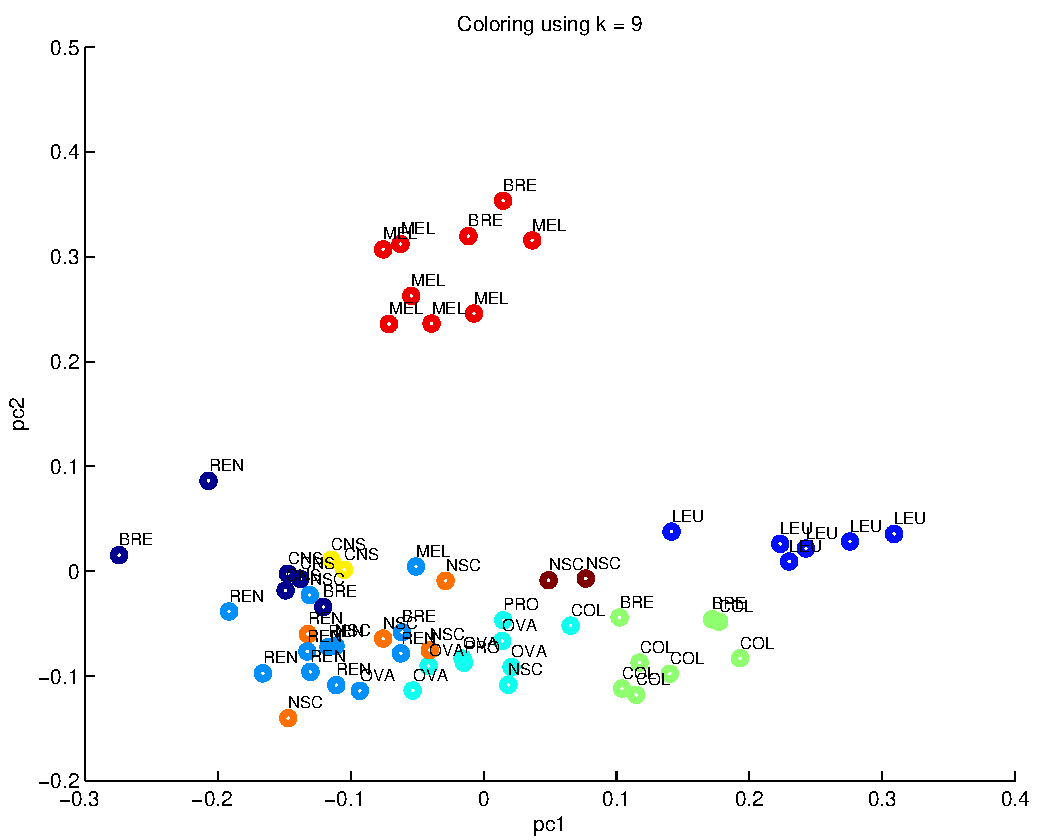
\includegraphics[width=0.95\textwidth]{./images/q34pcs2}
  \caption{2d plot according to pc$1$ and pc$2$ using k-means for
    coloring.}
  \label{fig:q34pcs2}
\end{figure}

\newpage

In figure \ref{fig:q34pcs3} can be seen using $k = 6$, the trend from
figure \ref{fig:q34pcs2} continues. \emph{NSC}, \emph{CNS}, \emph{OVA}
and \emph{BRE} seems intermixed in one big pile around pc$1$ $= -0.1$
and pc$2$ $= -0.05$. While the nicely clustered cancer groups from
figure \ref{fig:q34pcs2} again clusters nicely.

\begin{figure}[!htbp]
  \centering 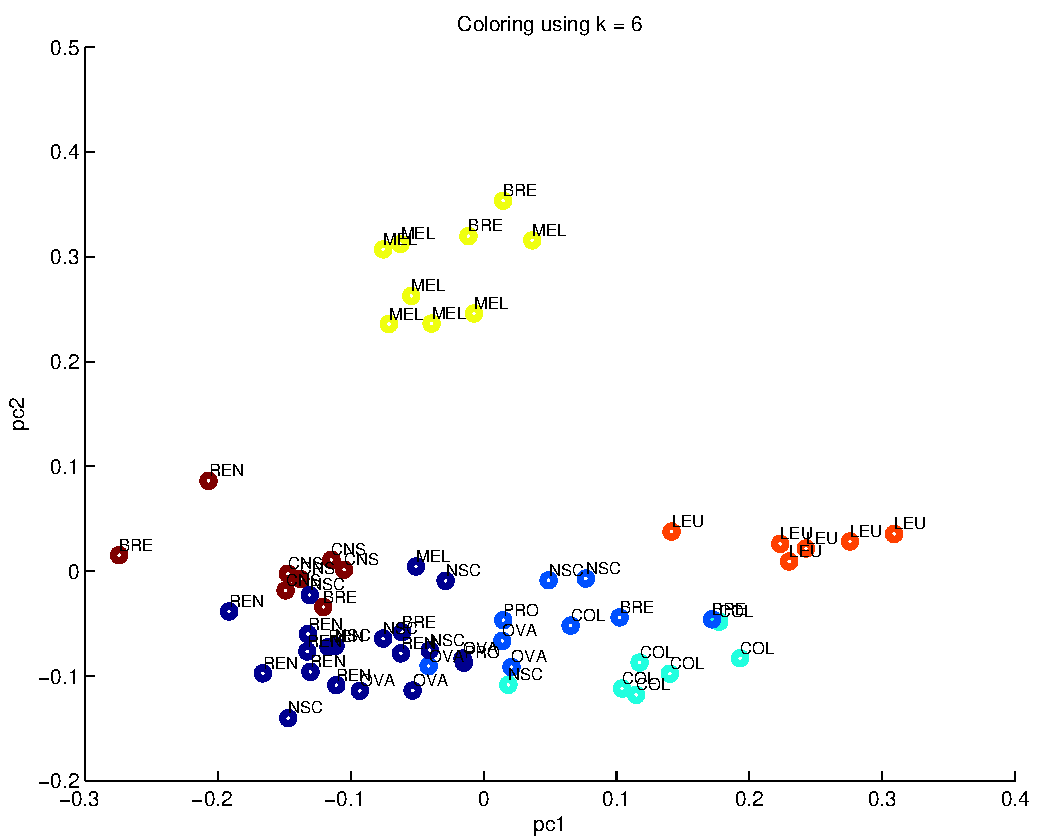
\includegraphics[width=0.95\textwidth]{./images/q34pcs3}
  \caption{2d plot according to pc$1$ and pc$2$ using k-means for
    coloring.}
  \label{fig:q34pcs3}
\end{figure}

\newpage

Here we now try to use the first three principal components to plot
the data in $3$d. To see if we can find out why some of the cancer
groups where so intermixed in the two previuos figures. As we can see
the cancer groups are still intermixed. We had hoped that using the
three first principal components we would have been able to make a
better seperation of the cancer groups.

\begin{figure}[!htbp]
  \centering 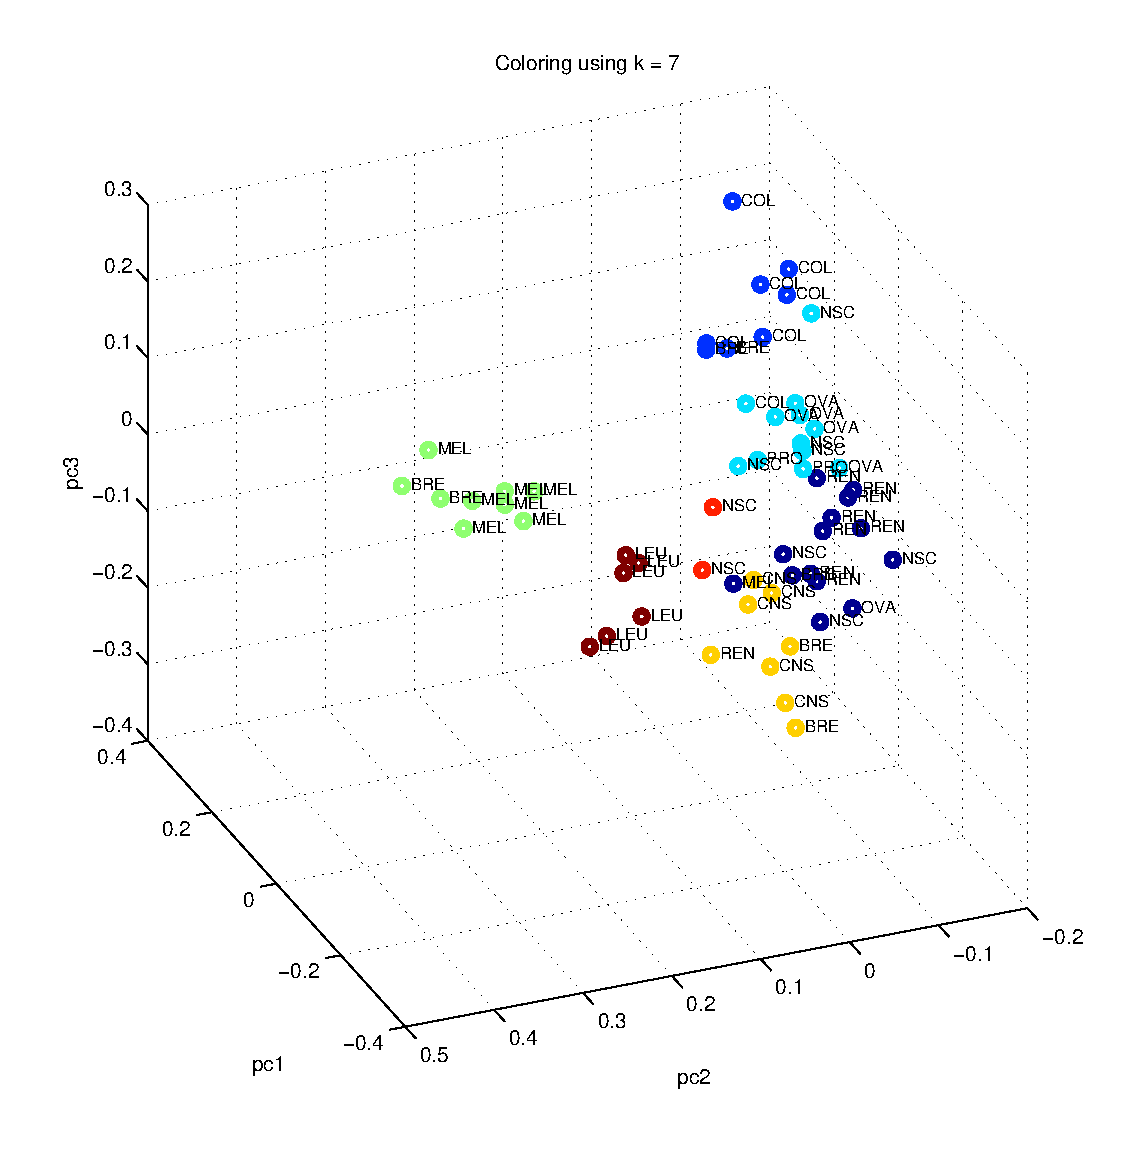
\includegraphics[width=0.95\textwidth]{./images/q34pcs4}
  \caption{3d plot according to pc$1$, pc$2$ and pc$3$ using k-means
    for coloring.}
  \label{fig:q34pcs4}
\end{figure}

From the above it seems like \emph{BRE} and \emph{NSC} are rather
heterogenous with its variance originating from other sources. And
with \emph{PRO} being homogenous with \emph{OVA}. Some of \emph{NSC}
(three cancer types) are also very much like \emph{OVA}.
